\section{Controle: lineariza\c{c}\~ao, resposta em frequ\^encia e projeto do PI}\label{sec:controle}

Arquivos: \arq{controle/linearizar_planta.m}, \arq{gvd_analitico.m}, \arq{resposta_freq.m},
\arq{margens.m}, \arq{projeto_pi.m}, \arq{resposta_degrau_mf.m}, \arq{lei_pi.m}. O MPPT n\~ao mexe na
raz\~ao c\'iclica $d$ diretamente: ele escolhe uma tens\~ao de refer\^encia $\Vref$, e um \textbf{PI de
tens\~ao} ajusta $d$ para que $\vpv$ siga $\Vref$. Este cap\'itulo mostra como esse PI foi projetado.

\subsection{A estrutura em dois la\c{c}os}

\begin{itemize}
\item \textbf{La\c{c}o interno (r\'apido):} PI que mede $\vpv$ e ajusta $d$ para seguir $\Vref$; escala de ms.
\item \textbf{La\c{c}o externo (lento):} MPPT que, a cada $\Ta$, escolhe um novo $\Vref$; escala de dezenas de ms.
\end{itemize}

\begin{figure}[htbp]
\centering
\begin{tikzpicture}
  \node[bloco,minimum width=1.6cm,minimum height=1.0cm] (mp) at (0,0) {MPPT};
  \node[circle,draw=cinza,thick,inner sep=1pt] (som) at (2.6,0) {$\Sigma$};
  \node[ctrl,minimum width=2.4cm] (pi) at (5.2,0) {PI\\{\scriptsize $K_p(1+\tfrac{1}{sT_i})$}};
  \node[bloco,minimum width=2.0cm] (atr) at (8.0,0) {Atraso PWM\\{\scriptsize $e^{-1{,}5sT_s}$}};
  \node[bloco,minimum width=2.4cm] (pl) at (11.0,0) {Planta\\{\scriptsize $-G_{vd}(s)$}};
  \draw[seta] (mp) -- node[rot,above]{$\Vref$} (som);
  \draw[seta] (som) -- node[rot,above]{$e$} (pi);
  \draw[seta] (pi) -- node[rot,above]{$d$} (atr);
  \draw[seta] (atr) -- (pl);
  \draw[seta] (pl.east) -- ++(0.7,0) node[rot,above right]{$\vpv$} -- ++(0,-1.5) -| node[rot,below,pos=0.2]{realimenta\c{c}\~ao de $\vpv$} (som.south);
  \draw[seta] ([xshift=0.7cm]pl.east) |- ($(mp.south)+(0,-2.2)$) -- (mp.south);
  \node[rot,anchor=north] at (3,-2.2) {mede $V,I$ a cada $\Ta$};
\end{tikzpicture}
\caption{Malha de tens\~ao do conversor. O ganho de malha \'e $L(s)=C(s)\,[-G_{vd}(s)]\,e^{-1{,}5sT_s}$; o sinal
negativo da planta \'e absorvido na defini\c{c}\~ao do erro.}
\label{fig:malha}
\end{figure}

O la\c{c}o externo s\'o funciona se o interno j\'a tiver acomodado quando o MPPT medir a pot\^encia: esse \'e o crit\'erio que
fixa $\Ta$ (Se\c{c}\~ao~\ref{sec:femia}).

\subsection{Lineariza\c{c}\~ao de pequenos sinais}

O modelo m\'edio \'e n\~ao linear (h\'a o produto $d\,i_L$ e a curva I-V do painel). Para projetar um controlador cl\'assico,
ele \'e linearizado em torno de um equil\'ibrio $(x_0,d_0)$, onde $f(x_0,d_0)=0$. Escreve-se $x=x_0+\tilde x$ e $d=d_0+\tilde d$
com $\tilde x$ e $\tilde d$ pequenos; a s\'erie de Taylor de 1.\textordmasculine\ ordem d\'a
\begin{equation}
\dot{\tilde x}=A\tilde x+B\tilde d,\qquad A=\frac{\partial f}{\partial x}\Big|_{(x_0,d_0)},\quad
B=\frac{\partial f}{\partial d}\Big|_{(x_0,d_0)},\quad \tilde v_{pv}=C\tilde x .
\end{equation}

\codigo{controle/linearizar_planta.m}{34}{80}{equil\'ibrio, matrizes $A$ e $B$ por diferen\c{c}as centrais e $r_{pv}$.}{lst:linear}

\begin{logica}
\begin{enumerate}
\item \textbf{Equil\'ibrio:} resolve o painel em \texttt{op.vpv} e acha $(d_0,i_{L0})$ com \arq{equilibrio_conversor}. Se o ponto for
 invi\'avel, d\'a erro dizendo se foi $\vpv>V_{oc}$ ou $d$ fora de $[D_{min},D_{max}]$.
\item \textbf{Matriz $A$:} perturba cada estado ($h=10^{-5}\max(1,|x_j|)$) e deriva por $(f(x_0+h)-f(x_0-h))/(2h)$, com erro $O(h^2)$.
 Assim a mesma fun\c{c}\~ao serve com ou sem perdas e para qualquer padr\~ao de sombra, sem derivar o painel \`a m\~ao.
\item \textbf{Vetor $B$:} idem, perturbando $d$ ($h=10^{-6}$).
\item \textbf{Resist\^encia din\^amica:} $r_{pv}=-1/(dI/dV)$. No MPP, $dP/dV=I+V\,dI/dV=0$ e $r_{pv}=V_{mp}/I_{mp}$: a din\^amica
 iguala a est\'atica; esse \'e o princ\'ipio do m\'etodo InC.
\item \textbf{CCM?} O modelo linear s\'o vale em condu\c{c}\~ao cont\'inua (\texttt{sys.ccm}).
\end{enumerate}
\end{logica}

\subsection{A planta $G_{vd}$ em forma fechada}

Sem perdas, com o painel virando um resistor $r_{pv}$, as equa\c{c}\~oes de pequenos sinais s\~ao
\begin{equation}
C\dot{\tilde v}=-\frac{\tilde v}{r_{pv}}-D\,\tilde i_L-I_L\,\tilde d,\qquad
L\dot{\tilde i}_L=D\,\tilde v+(V+V_{bat})\,\tilde d .
\end{equation}
Eliminando $\tilde i_L$ na transformada de Laplace:
\begin{equation}\label{eq:gvd}
G_{vd}(s)=\frac{\tilde v_{pv}}{\tilde d}=-\frac{L I_L\,s+D\,(V+V_{bat})}{L C\,s^2+(L/r_{pv})\,s+D^2}
\end{equation}

\codigointeiro{controle/gvd_analitico.m}{$G_{vd}(j\omega)$ sem perdas, para conferir a planta num\'erica.}{lst:gvd}

Tr\^es pontos de leitura:
\begin{itemize}
\item \textbf{Sinal negativo:} mais $d$ = chave mais tempo ligada; o indutor puxa mais corrente do capacitor e $\vpv$ cai.
\item \textbf{Polos:} $\omega_0=D/\sqrt{LC}$ e $\zeta=\sqrt{L/C}/(2D\,r_{pv})$. Com os valores do projeto isso d\'a a
 resson\^ancia LC em $\sim$240\,Hz, pouco amortecida ($\zeta$ de 0,16 a 0,3).
\item \textbf{Amortecimento:} o \'unico ``resistor'' do caso sem perdas \'e o pr\'oprio painel.
\end{itemize}

\codigointeiro{controle/resposta_freq.m}{$H(j\omega)=C(j\omega I-A)^{-1}B+D$, no lugar de \texttt{bode}/\texttt{freqresp}.}{lst:rfreq}

\subsection{Margens de estabilidade sem toolbox}

\texttt{margens(w,L)} substitui \texttt{margin()}. Duas defini\c{c}\~oes:
\begin{itemize}
\item \textbf{Margem de fase (MF):} na frequ\^encia $\omega_c$ onde $|L|=1$, quanto falta para a fase chegar a $-180^\circ$:
 $\mathrm{MF}=180^\circ+\angle L(j\omega_c)$. Se a fase chegasse a $-180^\circ$ com $|L|=1$, $L=-1$ e $1+L=0$: polo de malha
 fechada sobre o eixo imagin\'ario (oscila\c{c}\~ao sustentada). O usual \'e MF $\ge45^\circ$.
\item \textbf{Margem de ganho (MG):} na frequ\^encia onde a fase vale $-180^\circ$, quanto o ganho poderia crescer at\'e
 $|L|=1$: $\mathrm{MG}=-20\log_{10}|L(j\omega_{180})|$. MG $\ge6$\,dB significa que o ganho da planta pode dobrar sem instabilizar.
\end{itemize}

\codigointeiro{controle/margens.m}{margens de fase e ganho a partir de $L(j\omega)$ amostrado.}{lst:margens}

\begin{logica}
\begin{enumerate}
\item \texttt{fase = unwrap(angle(L))*180/pi}: fase cont\'inua, sem saltos de $360^\circ$.
\item \textbf{Cruzamentos de ganho:} varre as amostras e detecta onde $|L|$ passa de $\ge1$ para $<1$ (ou volta). Interpola em
 $\log|L|$, pois no Bode o m\'odulo varia como pot\^encia de $\omega$.
\item \textbf{Cruzamentos de fase:} detecta onde $\text{fase}+180^\circ$ muda de sinal (descartando o salto artificial de $\pm180^\circ$).
\item O c\'odigo olha \textbf{todos} os cruzamentos, n\~ao s\'o o primeiro, e fica com a pior margem: a resson\^ancia LC pode
 fazer $|L|$ voltar a passar de 1 depois do primeiro cruzamento.
\end{enumerate}
\end{logica}

\subsection{O projeto do PI (D12 e D13)}

O controlador \'e $C(s)=K_p(1+1/(sT_i))$, aplicado como $d=K_p(e+\xi/T_i)$ com $e=\vpv-\Vref$ e $\dot\xi=e$.

\begin{atencao}[: por que a regra cl\'assica falha]
A regra usual p\~oe o zero do PI uma d\'ecada abaixo do cruzamento ($\omega_z=\omega_c/5$, $r=0{,}2$). Aqui a planta \'e plana
(40 a 85\,V por unidade de $d$) at\'e a resson\^ancia LC. Com o zero abaixo de $\omega_c$, acima dele o PI vira praticamente s\'o o
ganho $K_p$, e $|L|$ fica perto de 1 desde $\omega_c$ at\'e a resson\^ancia: o pico cruza 0\,dB de novo com fase
$\approx-150^\circ$, e a MF cai para 25 a $40^\circ$. Subir $f_c$ acima da resson\^ancia tamb\'em n\~ao adianta: ali a fase da planta j\'a
est\'a perto de $-180^\circ$.
\end{atencao}

\textbf{O que funciona:} zero \emph{acima} do cruzamento ($r>1$). Abaixo do zero o PI age como integrador puro, $|L|$ cai
20\,dB/d\'ecada, o cruzamento fica bem abaixo da resson\^ancia e $|L|\ll1$ no pico LC. A fase em $\omega_c$ \'e $\approx-90^\circ$, ent\~ao a
MF \'e alta.

\codigo{controle/projeto_pi.m}{114}{170}{varredura de $f_c$ e $r$, escolha do maior $f_c$ que passa e c\'alculo de $\Ta$.}{lst:projpi}

\begin{logica}
\begin{enumerate}
\item Antes deste trecho, o c\'odigo monta os casos de robustez (pr\'oxima subse\c{c}\~ao) e lineariza cada um uma s\'o vez: a planta
 n\~ao depende do PI.
\item Para cada $f_c$ (80 valores, de 5\,Hz a $f_s/10$, espa\c{c}ados em log) e cada $r\in\{0{,}2;0{,}5;1;2;5\}$:
 \texttt{Ti = 1/(r*wc)} e \texttt{Kp} tal que $|L(j\omega_c)|=1$ no ponto nominal.
\item Calcula MF e MG em todos os casos. Se alguma ficar abaixo de $45^\circ$ ou 6\,dB, descarta o par.
\item Para os que passam, simula o degrau de $\Vref$ em cada caso (\texttt{resposta\_degrau\_mf}) e calcula $t_s$ (faixa de 2\,\%).
 Exige $t_{s,max}<50$\,ms, s\'o para rejeitar malhas absurdamente lentas.
\item Entre os aprovados, fica o de \textbf{maior $f_c$} (empate: maior MF): banda maior = malha mais r\'apida = passos de MPPT mais curtos.
\item No fim, $\Ta=1{,}5\,t_{s,max}$ arredondado para cima em ms.
\end{enumerate}
\end{logica}

\subsection{Robustez}

Indutores e capacitores eletrol\'iticos t\^em toler\^ancia t\'ipica de $\pm20$\,\%. Por isso cada ponto de opera\c{c}\~ao \'e
verificado com $L$ e $C$ nominais e nos cantos $[f_L\ f_C]=[1{,}2\ 1],[1\ 1{,}2],[1{,}2\ 1{,}2],[0{,}8\ 0{,}8]$. S\~ao 12 pontos de
opera\c{c}\~ao:
\begin{itemize}
\item 1000, 600 e 200\,W/m$^2$ uniformes, cada um no MPP e em $0{,}8V_{mp}$ e $1{,}1V_{mp}$ (o MPPT passeia em torno do MPP e o ganho muda com $r_{pv}$);
\item os dois picos da curva com um subm\'odulo a 400\,W/m$^2$;
\item o m\'odulo quente (60\,$^\circ$C, 1000\,W/m$^2$) no seu MPP.
\end{itemize}
S\~ao $12\times5=60$ casos. Em 4 deles, em 200\,W/m$^2$, o conversor cai em DCM e eles s\~ao exclu\'idos (o modelo linear de CCM
n\~ao vale ali); s\~ao conferidos depois na simula\c{c}\~ao n\~ao linear. O PI projetado s\'o com $L$ e $C$ nominais tinha MG de 4,6\,dB
com $L+20$\,\%, e por isso a robustez entrou no projeto.

\subsection{Resultado e per\'iodo do MPPT}\label{sec:femia}

\begin{resultado}
\small\centering
\begin{tabular}{@{}lc@{}}
\toprule
Grandeza & Valor \\ \midrule
Banda de cruzamento $f_c$ & 56,6\,Hz \\
Posi\c{c}\~ao do zero $r=\omega_z/\omega_c$ & 5 \\
$K_p$ & $2{,}5\times10^{-3}$\,V$^{-1}$ \\
$T_i$ & 0,562\,ms \\
Casos verificados em CCM & 56 de 60 \\
Pior MG nos 56 casos & 6,2\,dB (limita a banda; caso cr\'itico: 200\,W/m$^2$, $L+20$\,\%) \\
Pior $t_s$ (2\,\%) & 20,2\,ms \\
Per\'iodo do MPPT $\Ta=1{,}5\,t_{s,max}$ & 31\,ms \\
\bottomrule
\end{tabular}
\end{resultado}

A MG de 6,2\,dB \'e o que limita a banda. O pior $t_s$ vem do pico de baixa tens\~ao com sombra: o ganho DC da planta \'e $\sim$0,6 do nominal e,
como $K_p$ \'e fixado no nominal, o cruzamento cai na mesma propor\c{c}\~ao. Escalonar o ganho (um $K_p$ por ponto) tiraria essa
limita\c{c}\~ao, mas ficou fora do escopo.

\begin{intuicao}[: crit\'erio de Femia]
O P\&O compara a pot\^encia antes e depois de cada passo de $\Vref$. Se $\Ta$ for menor que o tempo de acomoda\c{c}\~ao da malha, a pot\^encia
medida ainda inclui o transit\'orio e o P\&O confunde essa din\^amica com uma mudan\c{c}a real de pot\^encia, podendo andar para o lado
errado. Por isso $\Ta>t_s$ no pior caso; o c\'odigo usa $1{,}5\,t_{s,max}$.
\end{intuicao}

\begin{figure}[htbp]
\centering
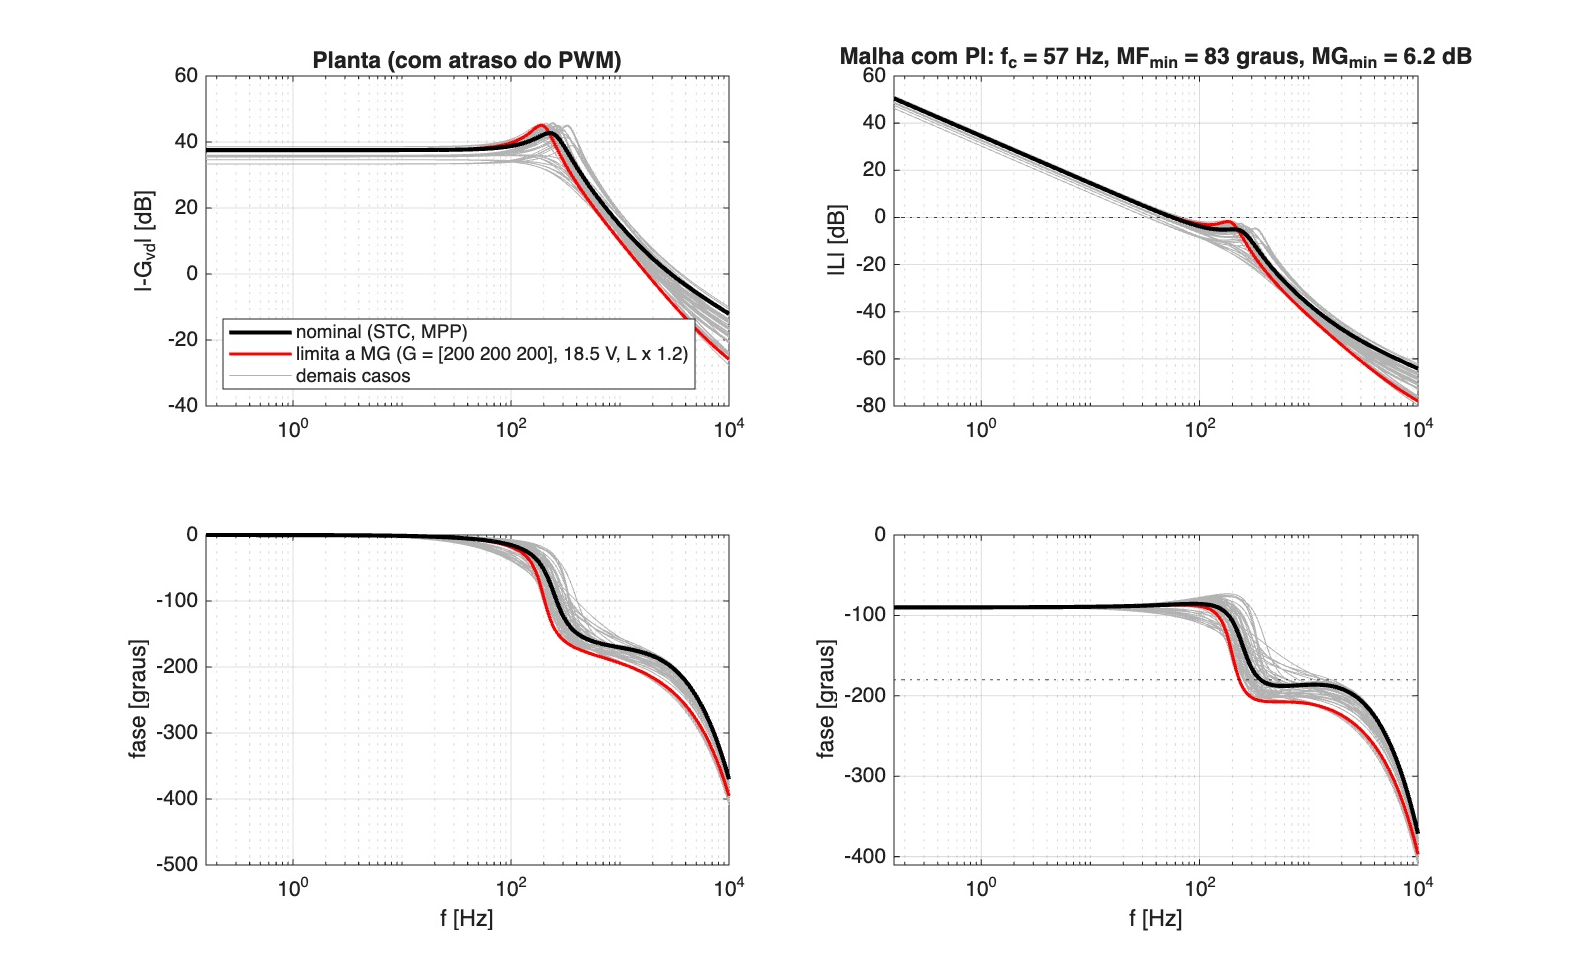
\includegraphics[width=0.95\linewidth]{e4_bode.pdf}
\caption{E4. Bode da planta e do ganho de malha com o PI. Preto: caso nominal; vermelho: o caso que limita a MG; cinza: os demais.}
\label{fig:e4bode}
\end{figure}

\begin{figure}[htbp]
\centering
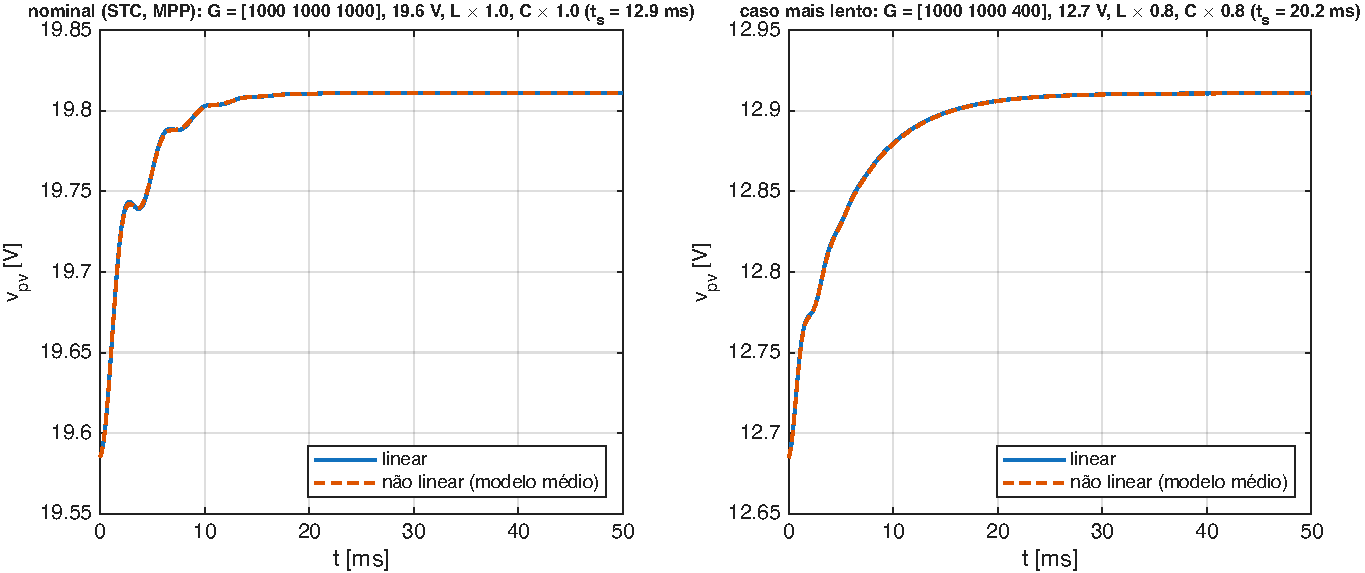
\includegraphics[width=0.9\linewidth]{e4_degrau.pdf}
\caption{E4. Degrau de $\Vref$: modelo linear (usado no projeto) contra o modelo m\'edio n\~ao linear.}
\label{fig:e4degrau}
\end{figure}

\subsection{A lei de controle com satura\c{c}\~ao}

\codigointeiro{controle/lei_pi.m}{PI de tens\~ao com satura\c{c}\~ao e anti-windup.}{lst:leipi}

\begin{logica}
\begin{enumerate}
\item $d=K_p(\text{err}+\xi/T_i)$, saturado em $[D_{min},D_{max}]=[0{,}02;\,0{,}95]$.
\item \textbf{Anti-windup:} com $d$ saturado, o integrador para se o erro empurrar o comando ainda mais para fora da faixa.
 Sem isso, $\xi$ cresceria sem limite e a malha demoraria a sair da satura\c{c}\~ao.
\item O argumento \texttt{modo} permite congelar a l\'ogica de satura\c{c}\~ao; \'e usado nos jacobianos por diferen\c{c}as finitas, para o
 passo n\~ao atravessar a descontinuidade.
\item A mesma fun\c{c}\~ao serve \`a simula\c{c}\~ao din\^amica e \`a quase-est\'atica: as duas usam exatamente o mesmo controle.
\end{enumerate}
\end{logica}
